% Anforderungen  an  Stabilität,  Robustheit,  Leistungsfähigkeit  etc.  des Systems.  Dies  beinhaltet  auch  den  Umgang  mit  fehlerhaften  Eingabedaten  oder  fehlerhaften Konfigurationen.
\section{Übersicht}
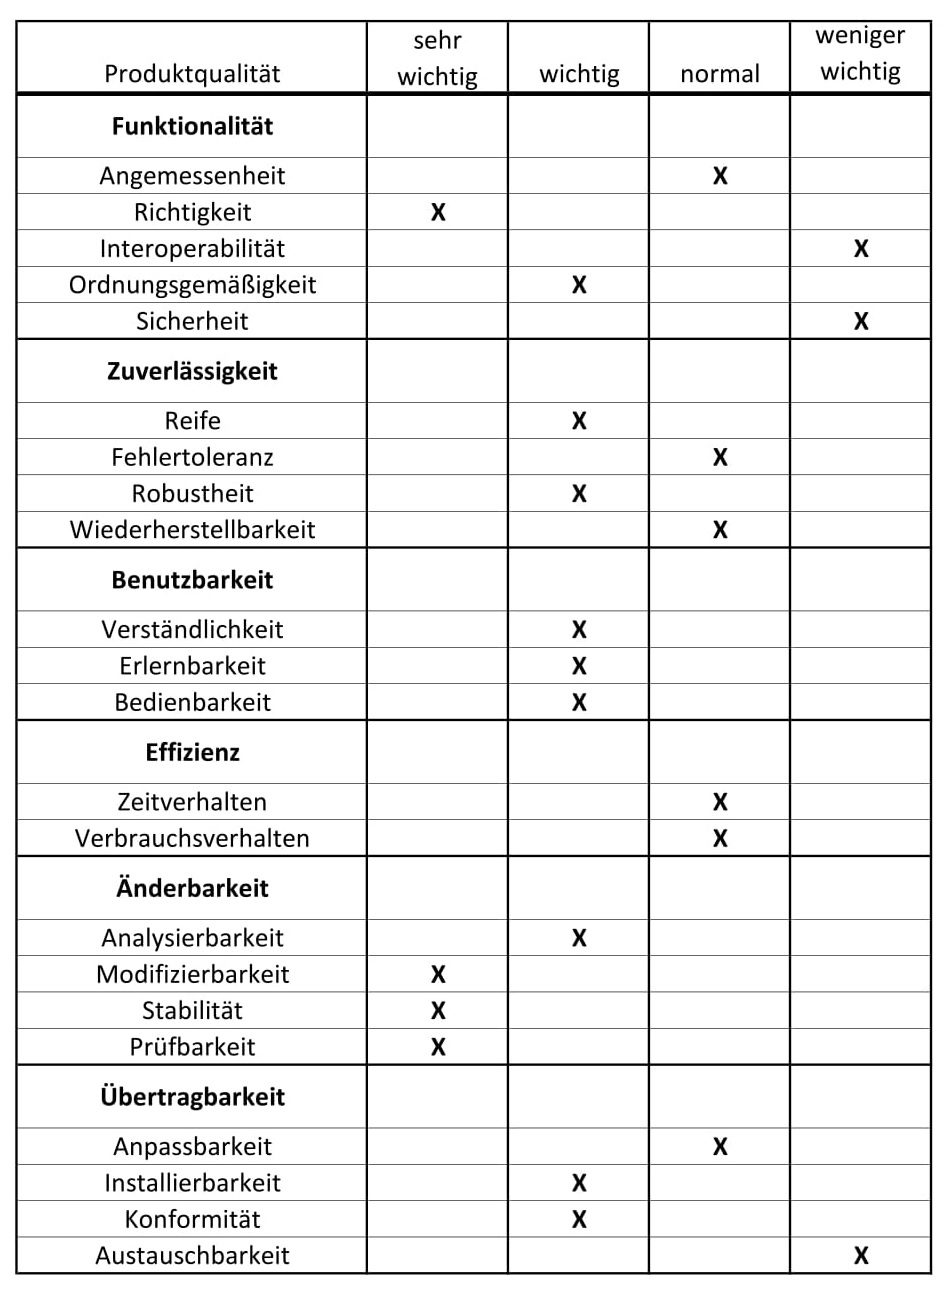
\includegraphics[scale=0.5]{img/Quali.jpg} 
\section{Zusammenfassung}
\begin{itemize}
\item Der Hautfokus der Software liegt auf korrekter Funktionsweise und Erweiterungen mit Hilfe von Plugins (Hauptsächlich weiter Algorithmen und Workflows).  
\item wichtige Qualitätsmerkmale sind gute Bedienbarkeit bei fachlichen Verständnis und Zuverlässigkeit, solange funktionstüchtige Algorithmen verwendet werden. Außerdem soll das Programm ohne großen Aufwand auf einem Linux-System installierbar sein.
\item Die Effizienz des Programms ist kaum beeinflussbar, da sie hauptsächlich von den verwendeten Algorithmen und Parameter dieser abhängt.
\item Sicherheit, Interoperabilität und Austauschbarkeit werden als weniger Wichtig erachtet, da das Programm eigenständig und auf einzelnen Computern ausgeführt wird.
\end{itemize}